%-------------------------------%
%  Author: Alessandro Sciarra   %
%    Date: 19 Oct 2020          %
%-------------------------------%

%~~~~~~~~~~~~~~~~~~~~~~~~~~~~~~~~~~~~~~~~~~~~%
\begin{frame}{Medium to large Bash projects I worked on}
    \large
    \addtolength{\leftmargini}{2em}
    \begin{columns}[T]
        \begin{column}{0.45\textwidth}
            \begin{uncoverenv}<2->
                \begin{enumerate}
                    \item \texttt{BaHaMAS}
                    \item GitHooks
                    \item BashLogger
                    \item SMASH-vHLLE-hybrid
                    \item \textcolor{bg!85!normal text.fg}{Coffee machine handler}
                \end{enumerate}
            \end{uncoverenv}
        \end{column}
        \begin{column}{0.45\textwidth}
            \centering
            \uncover<3>{
\includegraphics[width=0.6\textwidth]{Showoff}}
        \end{column}
    \end{columns}
    \begin{tikzpicture}[remember picture, overlay]
        \begin{DrawOnNode}{current page}
            \node at (0.5, 0.26) {
\includegraphics[width=0.5\textwidth]{Bash-is-enough}};
        \end{DrawOnNode}
    \end{tikzpicture}
\end{frame}
%~~~~~~~~~~~~~~~~~~~~~~~~~~~~~~~~~~~~~~~~~~~~%
\begingroup
    \newcommand{\bahamas}{\texttt{BaHaMAS}}
    \usebackgroundtemplate{
\includegraphics[height=\paperheight]{BHMAS_Frontpage}}
    \begin{frame}%[plain, noframenumbering, hideframenumber]
        \PrepareURLsymbol[PS]
        \begin{tikzpicture}[overlay, remember picture]
            \node[text=PP, anchor=north, align=center, font=\LARGE] (title) at ([shift={(1cm,-3mm)}]current page.north) {\bahamas};
            \node[text=PB, below = 0mm of title] (subtitle) {A \texttt{Ba}sh \texttt{Ha}ndler to \texttt{M}onitor and \texttt{A}dministrate \texttt{S}imulations};
            \begin{scope}[scope on=<2>]
                \node[below = 5mm of subtitle.south west, anchor=north west, xshift=-12mm] {
                    \begin{minipage}{0.85\textwidth}
                        \begin{itemize}
                            \item It is a \URL*{https://github.com/AG-Philipsen/BaHaMAS}{publicly available software} to support LQCD practitioners' work
                            \item An example of huge Bash project, $\mathcal{O}$(10$^\text{4}$) lines of code
                            \item Actually, kind of many executables handled by the same main script
                            \item Everything achieved via handy git-inspired command line options
                            \item Interactive setup and command line autocompletion available
                            \item Functional tests only (almost 100, though)
                            \item Partial system requirements validation at start-up
                            \item Manual pages for in terminal documentation
                            \item Online Wiki documentation for general overview
                        \end{itemize}
                    \end{minipage}
                };
            \end{scope}
            \begin{scope}[scope on=<3>]
                \draw(subtitle.south) +(0,-5mm) -- ++(0,-55mm) node[yshift=-1cm, xshift=-3mm, text=PB]
                        {\ldots{}after all, \bahamas{} is a good name...};
                \path coordinate (L) at ($(subtitle.south west)!0.4!(subtitle.south)$)
                      coordinate (R) at ($(subtitle.south east)!0.4!(subtitle.south)$);
                \node[below = 7mm of L] (L1) {
\includegraphics[height=21mm]{BHMAS_Flag}};
                \node[below = 7mm of R] (R1) {
\includegraphics[height=21mm]{BHMAS_Logo}};
                \node[below = 5mm of L1, xshift=3mm, font=\footnotesize] (L2) {
                    \begin{minipage}{48mm}
                        \begin{itemize}
                            \item You can freely run on beaches
                            \item You have a lot of free time
                            \item Cocktails help in relaxing
                        \end{itemize}
                    \end{minipage}
                };
                \node[below = 5mm of R1, xshift=3mm, font=\footnotesize] (R2) {
                    \begin{minipage}{48mm}
                        \begin{itemize}
                            \item You can \PB{\emph{effectively}} run on clusters
                            \item You \PB{\emph{get}} a lot of free time
                            \item Cocktails \PB{\emph{may}} help in developing
                        \end{itemize}
                    \end{minipage}
                };
            \end{scope}
        \end{tikzpicture}
    \end{frame}
\endgroup
%~~~~~~~~~~~~~~~~~~~~~~~~~~~~~~~~~~~~~~~~~~~~%
\begin{frame}{A more generic project: \URL[PB]{https://github.com/AxelKrypton/GitHooks}{GitHooks}}
    \begin{varblock}{quote}[0.9\textwidth]{What is it about?}
        This small collection of bash script is an attempt to have a git-repository-independent hooks setup mechanism to comfortably use over and over again the own implemented hooks.
        The basic idea is to have a general hooks implementation and a bash main script to set up them in any git repository with command line options to fine tune the setup.
        All provided hooks and setup have a highly informative output.
    \end{varblock}
    \vspace{2mm}
    \begin{itemize}
        \item Giving it a try should be straightforward
        \item It helps you keeping \PP{history of your repositories tidy} \Remark{via the \;\texttt{commit-msg}\; hook}
        \item It helps you keeping \PS{the code in your repositories tidy}, optionally \Remark{via the \;\texttt{pre-commit}\; hook}
              \begin{itemize}
                  \item checking C++ code style using clang-format
                  \item checking copyright statement
                  \item checking license notice
              \end{itemize}
    \end{itemize}
\end{frame}
%~~~~~~~~~~~~~~~~~~~~~~~~~~~~~~~~~~~~~~~~~~~~%
\begin{frame}[fragile]{A wide-audience support script: \URL[PB]{https://github.com/AxelKrypton/BashLogger}{A Bash Logger}}
    \vspace{-2mm}
    \begin{overlayarea}{\textwidth}{0.8\textheight}
        \begin{itemize}[<only@1-2>]
            \setlength{\itemsep}{4pt}
            \item Extremely simple to use and/or to include in your project
            \item It allows to unify the style of all your output messages
            \item Errors are redirected to the standard error as it should be
            \item Messages are classified in levels which can be easily switched on or off at run-time
            \item Messages are printed to a given file descriptor (customizable at source time)\\
                  \Then{Logger still usable in functions whose ``return value'' is printed to standard output and meant to be captured by command substitution}
            \item Fatal errors exit with a given exit code (customizable at source time)\\
                  \Then{Customization also possible on single usage, e.g.\\
                  \colorbox{background-color}{\scriptsize\bash|exit_code=42 Print_Fatal_And_Exit 'Houston, we have a problem!'|}}
            \item Super cool automatic highlighting mechanism
        \end{itemize}
        \begin{onlyenv}<2>
            \begin{lstlisting}[style=myBash, aboveskip=3mm, numbers=none]
                $ git clone https://github.com/AxelKrypton/BashLogger
                # ...
                $ emacs -nw TestLogger.bash
            \end{lstlisting}
        \end{onlyenv}
        \begin{onlyenv}<3>
            \begin{lstlisting}[style=myBash, aboveskip=0mm, numbers=none, style=smaller, xleftmargin=0mm, xrightmargin=0mm]
                #!/usr/bin/env bash
                #
                #  Copyright (c) 2019 Alessandro Sciarra <sciarra@itp.uni-frankfurt.de>
                #
                #  This file is part of BashLogger.
                #
                #  [...]
                #

                trap 'printf "\n"' EXIT
                source Logger.bash "$@" || exit 1

                Print_Trace              '\nTrace message '       --emph 'highlighted' ' VS normal'
                Print_Debug              '\nDebug message '       --emph 'highlighted' ' VS normal'
                Print_Info               '\nInformation message ' --emph 'highlighted' ' VS normal'
                Print_Info               '\nTrailing' '--emph'
                Print_Info               --emph '--emph'
                Print_Info               --emph
                Print_Info               ''
                Print_Attention          '\n' 'Attention message '   --emph 'highlighted' ' VS normal'
                Print_Warning            '\n' 'Warning message '     --emph 'highlighted' ' VS normal'
                Print_Error              '\n' 'Error '               --emph 'highlighted' ' VS normal'
                ( Print_Fatal_And_Exit   '\n' 'Fatal error exit! '   --emph 'highlighted' ' VS normal' )
                Print_Internal_And_Exit  '\n' 'Developer error '     --emph 'highlighted' ' VS normal'
            \end{lstlisting}
        \end{onlyenv}
        \begin{onlyenv}<4-5>
            \vspace{-4mm}
            \begin{center}
                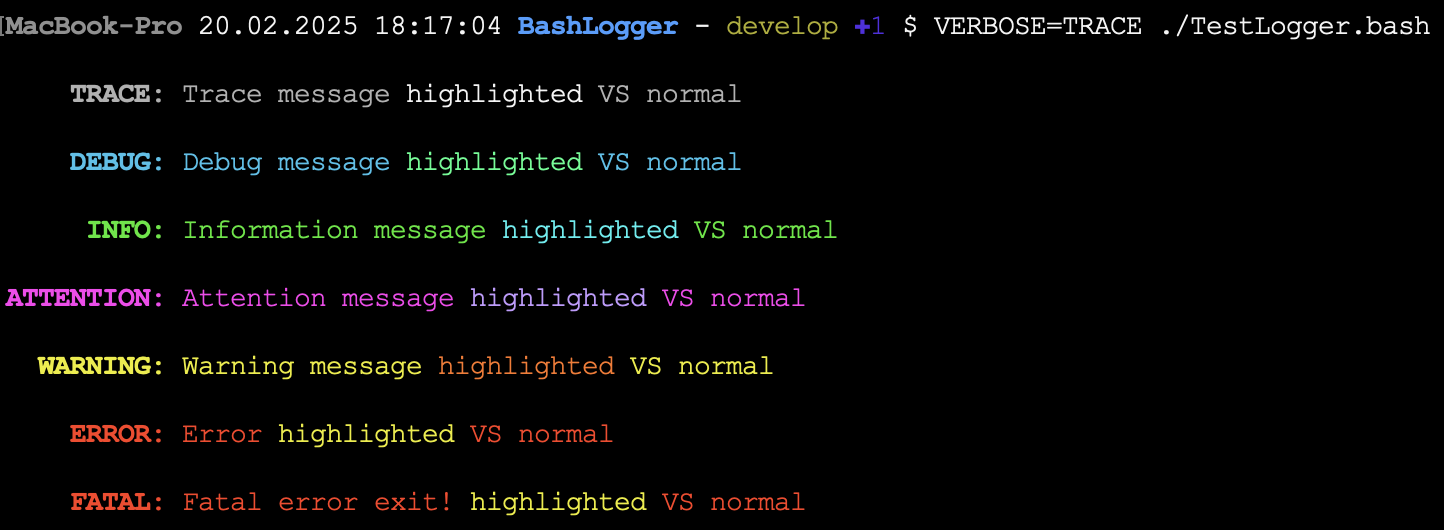
\includegraphics[width=0.88\textwidth]{BashLogger_output}\\[-1pt]
                \uncover<5>{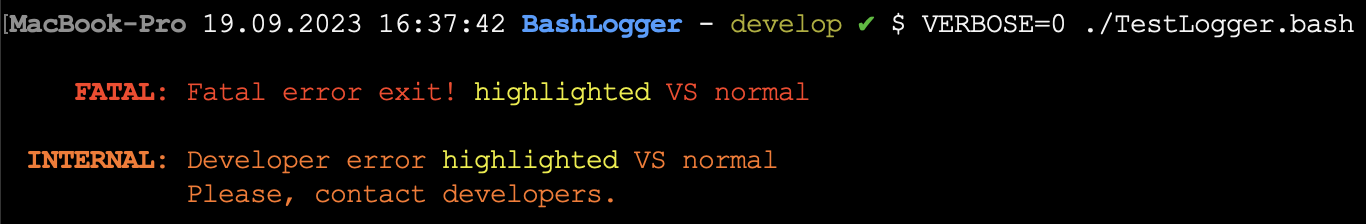
\includegraphics[width=0.88\textwidth]{BashLogger_output_minimal}}
            \end{center}
        \end{onlyenv}
    \end{overlayarea}
    \FrameRemark{For a detailed description of all functionality refer to the README file of the project.}
\end{frame}
%~~~~~~~~~~~~~~~~~~~~~~~~~~~~~~~~~~~~~~~~~~~~%
\begin{frame}[fragile]{Another remarkable handler: \URL[PB]{https://smash-transport.github.io/smash-vhlle-hybrid/develop/}{SMASH-vHLLE-Hybrid}}
    \begin{center}
        \includegraphics[width=\textwidth]{SMASH-vHLLE-Hybrid}
    \end{center}
    \begin{itemize}
        \item Another example of large Bash project, $\mathcal{O}$(10$^\text{4}$) lines of code
        \item Own test framework with unit and functional tests
        \item Appealing documentation of the project
    \end{itemize}
\end{frame}
%~~~~~~~~~~~~~~~~~~~~~~~~~~~~~~~~~~~~~~~~~~~~%
